\pagebreak
\section{Pianificazione}
\subsection{Verso la RTB}
\subsubsection{Primo periodo} 
Inizio: 8/11/2023 \\
Fine: 24/11/2023 \\

\textbf{}

\begin{tblr}{
    colspec={|X[5cm]|X[.5cm]|X[.5cm]|X[.5cm]|X[.5cm]|X[.5cm]|X[.5cm]|X[3.5cm]},
    row{odd}={bg=white},
    row{even}={bg=lightgray},
    row{1}={bg=black,fg=white},
    row{8}={bg=black,fg=white}
    }
    
    Nominativo & Re & Am & An & Pg & Pr & Vf & Ore Totali \\ \hline
    Alberto C.    & -  & -  & -  & 4  & -  & 1  & 5 \\ \hline
    Bilal El M.   & -  & -  & 4  & -  & -  & 1  & 5 \\ \hline
    Alberto M.    & 3  & 2  & -  & -  & -  & -  & 5 \\ \hline
    Alex S.       & 2  & 3  & -  & -  & -  & -  & 5 \\ \hline
    Iulius S.     & -  & -  & 4  & -  & -  & 1  & 5 \\ \hline
    Giovanni Z.   & -  & -  & -  & 4  & -  & 1  & 5 \\ \hline
    Totale        & 5  & 5  & 8  & 8  & 0  & 4  & 30 \\ \hline
    
\end{tblr}

\textbf{Preventivo economico}

\begin{tblr}{
colspec={|X[5cm]|X[3.5cm]|X[1.5cm]|X[3.5cm]},
row{odd}={bg=white},
row{even}={bg=lightgray},
row{1}={bg=black,fg=white},
row{8}={bg=black,fg=white}
}

Ruolo & Costo orario (€/h) & N. Ore & Costo totale (€)  \\ \hline
Responsabile      & 30,00 &  5  &   150,00 \\ \hline
Amministratore    & 20,00 &  5  &   100,00 \\ \hline
Analista          & 25,00 &   8 &   200,00 \\ \hline
Progettista       & 25,00 &   8 &   200,00 \\ \hline
Programmatore     & 15,00 &   0 &     0,00 \\ \hline
Verificatore      & 15,00 &   4 &    60,00 \\ \hline
Totale & \SetCell[c=1]{c} &  30 &   710,00 \\ \hline

\end{tblr}

\paragraph{Attività svolte} 
\subparagraph{}
Le attività svolte dai membri del gruppo nel primo periodo sono state:
\begin{itemize}
    \item Concepimento della prima versione del Way of Working$^{G}$;
    \item Ricerca bibliografica finalizzata a costruire il body of knowledge necessario alla comprensione della documentazione
    che dovrà essere prodotta nella fase di RTB;
    \item Studio dei seguenti documenti:
    \begin{itemize}
        \item ISO/IEC 12207 : Processi del ciclo di vita del software;
        \item ISO/IEC TR 19759: Software Engineering - Guide to the Software Engineering Body of Knowledge; 
        \item IEEE 830: Pratiche raccomandate per la specifica dei requisiti software;
    \end{itemize}
    \item Ricerca delle tecnologie potenzialmente adatte ad essere incluse nello
    stack tecnologico e loro studio;
    \item Individuazione delle tecnologie di supporto nella produzione di documenti; 
    \item Individuazione delle tecnologie di supporto nel versionamento dei documenti e del codice prodotto
    successivamente durante la codifica del PoC$^{G}$.
\end{itemize}

\graphicspath{ {./src/Gantt/} } 

\begin{figure}[h] 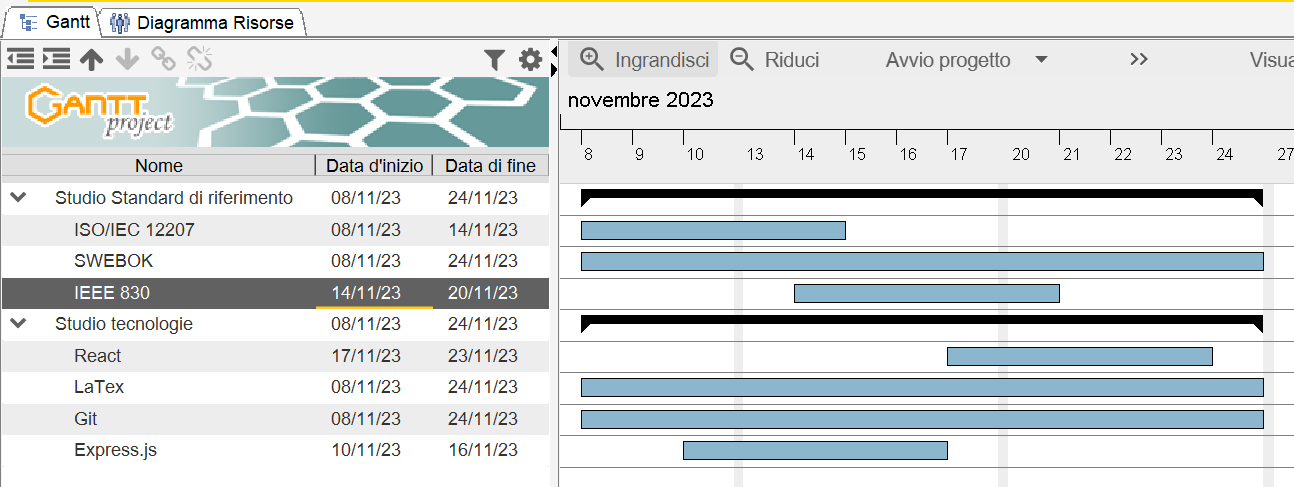
\includegraphics[scale=.6]{GanttPrimoPeriodo.png} \end{figure}

\textbf{Consuntivo orario}

\begin{tblr}{
    colspec={|X[5cm]|X[.5cm]|X[.5cm]|X[.5cm]|X[.5cm]|X[.5cm]|X[.5cm]|X[3.5cm]},
    row{odd}={bg=white},
    row{even}={bg=lightgray},
    row{1}={bg=black,fg=white},
    row{8}={bg=black,fg=white}
    }
    
    Nominativo & Re & Am & An & Pg & Pr & Vf & Ore Totali \\ \hline
    Alberto C.    & -  & -  & -  & 4  & -  & 1  & 5 \\ \hline
    Bilal El M.   & -  & -  & 4  & -  & -  & 1  & 5 \\ \hline
    Alberto M.    & 3  & 2  & -  & -  & -  & -  & 5 \\ \hline
    Alex S.       & 2  & 3  & -  & -  & -  & -  & 5 \\ \hline
    Iulius S.     & -  & -  & 4  & -  & -  & 1  & 5 \\ \hline
    Giovanni Z.   & -  & -  & -  & 4  & -  & 1  & 5 \\ \hline
    Totale        & 5  & 5  & 8  & 8  & 0  & 4  & 30 \\ \hline

\end{tblr}

\textbf{Consuntivo economico}

\begin{tblr}{
colspec={|X[5cm]|X[3.5cm]|X[1.5cm]|X[3.5cm]},
row{odd}={bg=white},
row{even}={bg=lightgray},
row{1}={bg=black,fg=white},
row{8}={bg=black,fg=white}
}

Ruolo & Costo orario (€/h) & N. Ore & Costo totale (€)  \\ \hline
Responsabile      & 30,00 &  5  &   150,00 \\ \hline
Amministratore    & 20,00 &  5  &   100,00 \\ \hline
Analista          & 25,00 &   8 &   200,00 \\ \hline
Progettista       & 25,00 &   8 &   200,00 \\ \hline
Programmatore     & 15,00 &   0 &     0,00 \\ \hline
Verificatore      & 15,00 &   4 &    60,00 \\ \hline
Totale & \SetCell[c=1]{c} &  30 &   710,00 \\ \hline

\end{tblr}

\textbf{Gestione dei ruoli}
\paragraph{}
In questo primo periodo,il 26\% delle ore di lavoro sono state dedicate alla fase di analisi,
data la necessità di effettuare uno studio preliminare dei documenti che dovranno essere prodotti durante
l'arco del progetto (in particolare le Norme di Progetto e il Piano di Progetto) e quindi dei relativi Standard
internazionali di riferimento; un'eguale percentuale di risorse orarie è stata spesa per il ruolo di Progettista, per ricercare, individuare e studiare le teconologie
potenzialmente adatte al prodotto da sviluppare; il 16\% delle ore è stato dedicato al ruolo del Responsabile, in cui si sono mossi i primi 
passi nell'ambito della gestione ed organizzazione del carico di lavoro tra i vari membri; un'eguale percentuale di ore 
è stata spesa per il ruolo di Amministratore il quale si è occupato dell'organizzazione della repository sulla piattaforma GitHub; infine il 12\% delle ore è stato dedicato al ruolo di Verificatore,
durante le quali i membri hanno preso dimestichezza con l'operazione di verifica e validazione dei primi documenti prodotti.

\paragraph{Gestione dei rischi}

\begin{itemize}
\item \textbf{Rischio verificatosi:} Scarsa esperienza tecnologica.
\begin{itemize}
\item \textbf{Esito Piano di Contingenza:} Tramite lo studio individuale e soprattutto tramite la trasmissione di conoscenza dai membri maggiormente esperti nel linguaggio LaTex e nei comdandi Git
a quelli meno esperti, il gruppo è riuscito efficacemente a mettere in pratica il piano di contingenza previsto per il suddetto
rischio, ottenendo un allineamento delle conoscenze tra i veri membri.\\
\item \textbf{Impatto:} L'impatto della scarsa esperienza tecnologica è stato nullo in questo primo periodo, 
avendo il gruppo preventivato la necessità di dedicare innanzitutto risorse all'individuazione,allo studio e all'apprendimento
delle tecnologie di supporto, così come di quelle che andranno a far parte dello stack tecnologico del prodotto.\\ 
\end{itemize}
\end{itemize}

\paragraph{}
\textbf{Retrospettiva:} \\
In questo primo periodo, il gruppo ha speso la maggior parte delle proprie ore svolgendo un lavoro di ricerca ed analisi 
su due fronti, ovvero quello della documentazione e del Proof of Concept: per quanto concerne la prima, sono stati studiati gli standard internazioni di riferimento
con lo scopo di disegnare una mappa concettuale dei documenti che dovranno essere prodotti, in particolare delle Norme ed del Piano di Progetto; per quanto 
riguarda il PoC invece sono state individuate e studiate tecnologie potenzialmente adatte allo sviluppo del prodotto, e successivamente selezionate quelle utilizzate per il PoC stesso. Inoltre, grande attenzione si è spesa per la definizione di norme che regolino il Way of Working, data la presenza di studenti-lavoratori (con 
specifiche esigenze legate agli impegni extra-universitari) fra i membri del gruppo, e quindi la necessità di un'efficace ed efficiente gestione delle ore, della ripartizione dei ruoli
e della suddivisione dei tasks fra i membri stessi. Nonostante una buona definizione dei ruoli, il gruppo non è riuscito ancora ad individuare la modalità secondo la quale
ruotare in futuro i ruoli stessi.
\begin{itemize}
    \item \textbf{Obiettvi raggiunti:}
    \begin{itemize}
        \item Allineamento da parte del gruppo, delle conoscenze del linguaggio LaTex e dei comandi Git;
        \item Scelta delle tenologie da includere nello stack tecnologico;
        \item Inizio dell'analisi dei requisiti funzionali del prodotto;
    \end{itemize}
    \item \textbf{Obiettivi mancati:}
    \begin{itemize}
        \item Definizione della modalità di rotazione dei ruoli.
    \end{itemize}
\end{itemize}

\subsubsection{Secondo periodo} 
Inizio: 25/11/2023 \\
Fine: 26/01/2024 \\

\textbf{Preventivo orario}

\begin{tblr}{
    colspec={|X[5cm]|X[.5cm]|X[.5cm]|X[.5cm]|X[.5cm]|X[.5cm]|X[.5cm]|X[3.5cm]},
    row{odd}={bg=white},
    row{even}={bg=lightgray},
    row{1}={bg=black,fg=white},
    row{8}={bg=black,fg=white}
    }
    
    Nominativo    & Re & Am & An & Pg & Pr & Vf & Ore Totali \\ \hline
    Alberto C.    & -  & -  & -  & -  & 15 & 2  & 17 \\ \hline
    Bibal El M.   & 2  & 3  & -  & 4  & -  & 2  & 11 \\ \hline
    Alberto M.    & 5  & -  & 5  & -  & -  & -  & 10 \\ \hline
    Alex S.       & -  & -  & -  & 5  & 5  & 5  & 15 \\ \hline
    Iulius S.     & -  & -  & 7  & -  & -  & 2  & 9  \\ \hline
    Giovanni Z.   & -  & -  & -  & -  & 10 & -  & 10 \\ \hline
    Totale        & 7  & 3  & 12 & 9  & 30 & 11 & 72 \\ \hline

\end{tblr}

\textbf{Preventivo economico}

\begin{tblr}{
colspec={|X[5cm]|X[3.5cm]|X[1.5cm]|X[3.5cm]},
row{odd}={bg=white},
row{even}={bg=lightgray},
row{1}={bg=black,fg=white},
row{8}={bg=black,fg=white}
}

Ruolo & Costo orario (€/h) & N. Ore & Costo totale (€)  \\ \hline
Responsabile      & 30,00 &  7  &   210,00 \\ \hline
Amministratore    & 20,00 &  3  &   60,00 \\ \hline
Analista          & 25,00 &  12 &   300,00 \\ \hline
Progettista       & 25,00 &  9  &   225,00 \\ \hline
Programmatore     & 15,00 &  30 &   450,00 \\ \hline
Verificatore      & 15,00 &  11 &   165,00 \\ \hline
Totale & \SetCell[c=1]{c} &  72 & 1.415,00 \\ \hline

\end{tblr}

\textbf{Attività svolte}

\paragraph{}Le attività svolte dal gruppo nel secondo periodo sono state:
\begin{itemize}
    \item Analisi dei rischi che possono verificarsi durante lo svolgimento dei processi 
    che compongono il progetto, e delle relative possibili strategie di mitigazione;
    \item In seguito all'individuazione delle tecnologie , progettazione e codifica del PoC;
    \item Colloquio con il prof. Cardin per ottenere delucidazioni riguardo lo studio dei requisiti funzionali;
    \item Prima stesura dei requisiti funzionali del prodotto da sviluppare;
    \item Prosieguo della stesura delle Norme di Progetto;
    \item Studio delle metriche da adottare al fine di misurare la qualità di prodotto e dei processi (particolare attenzione
    spesa per quest'ultimi);
    \item Webinar$^{G}$ organizzato dall'azienda proponente sull'utilizzo di Docker$^{G}$.
\end{itemize}

\graphicspath{ {./src/Gantt/} } 
\begin{figure}[h] 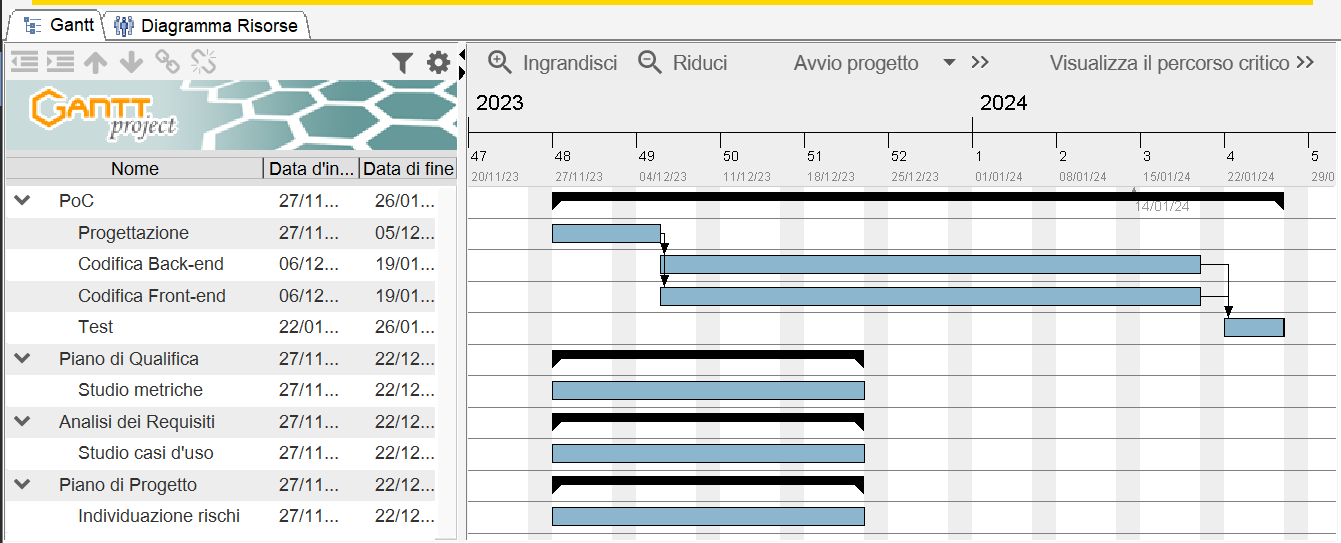
\includegraphics[scale=.6]{GanttSecondoPeriodo.png} \end{figure}

\textbf{Consuntivo orario}

\begin{tblr}{
    colspec={|X[5cm]|X[.5cm]|X[.5cm]|X[.5cm]|X[.5cm]|X[.5cm]|X[.5cm]|X[3.5cm]},
    row{odd}={bg=white},
    row{even}={bg=lightgray},
    row{1}={bg=black,fg=white},
    row{8}={bg=black,fg=white}
    }
    
    Nominativo    & Re & Am & An & Pg & Pr & Vf & Ore Totali \\ \hline
    Alberto C.    & -  & -  & -  & -  & 20 & 5  & 25 \\ \hline
    Bibal El M.   & -  & -  & -  & 4  & -  & 2  & 6  \\ \hline
    Alberto M.    & 2  & 3  & 5  & -  & -  & -  & 10 \\ \hline
    Alex S.       & -  & -  & -  & 5  & 5  & 5  & 15 \\ \hline
    Iulius S.     & -  & -  & 3  & 4  & -  & 2  & 9  \\ \hline
    Giovanni Z.   & -  & -  & -  & -  & 15 & -  & 15 \\ \hline
    Totale        & 2  & 3  & 8  & 13 & 40 & 14 & 80\\ \hline

\end{tblr}

\textbf{Consuntivo economico}

\begin{tblr}{
colspec={|X[5cm]|X[3.5cm]|X[1.5cm]|X[3.5cm]},
row{odd}={bg=white},
row{even}={bg=lightgray},
row{1}={bg=black,fg=white},
row{8}={bg=black,fg=white}
}

Ruolo & Costo orario (€/h) & N. Ore & Costo totale (€)  \\ \hline
Responsabile      & 30,00 &  2  &    60,00 \\ \hline
Amministratore    & 20,00 &  3  &    60,00 \\ \hline
Analista          & 25,00 &  8  &   200,00 \\ \hline
Progettista       & 25,00 &  13 &   325,00 \\ \hline
Programmatore     & 15,00 &  40 &   450,00 \\ \hline
Verificatore      & 15,00 &  14 &   165,00 \\ \hline
Totale & \SetCell[c=1]{c} &  80 & 1.260,00 \\ \hline

\end{tblr}

\textbf{Gestione dei ruoli}

\paragraph{}
Nel secondo periodo, il ruolo per il quale è stata spesa la fetta più consistente di ore (50\%),
è stato quello di Programmatore, data la volontà del gruppo di completare entro la fine del periodo 
la codifica del PoC e la relativa fase di test (alla quale è stato dedicato il 17\% delle ore);il 16\% delle risorse è stato dedicato alla figura del Progettista
per supportare e guidare i Programmatori nel lavoro di codifica; nonostante la necessità
di proseguire con la stesura della documentazione e con l'analisi dei requisiti funzionali, solo il 10\% delle ore è stato
dedicato al ruolo di Analista; il 3\% delle ore è stato dedicato  alla figura del Responsabile e il 3\%
dell'Amministratore.

\paragraph{Gestione dei rischi}

\begin{itemize}
\item \textbf{Rischio verificatosi:} Conflitti decisionali.

\begin{itemize}
\item \textbf{Esito Piano di Contingenza:}Essendosi presentati punti di vista differenti riguardo le tecnologie da includere nello stack ,sia per quanto riguarda la parte di Front-end  che quella di Back-end, i membri del gruppo 
hanno avviato una discussione nella quale considerare i pro e i contro delle differenti proposte; si è deciso di 
affidare la scelta definitiva ai membri con la maggior expertise nell'ambito dei linguaggi di programmazione.
\item \textbf{Impatto:} L'impatto è stato nullo, grazie alla disponibilità e alla maturità dimostrata da tutti i membri del gruppo
nell'affrontare un conflitto decisionale e soprattutto nell'accettarne la risoluzione.  
\end{itemize}

\item \textbf{Rischio verificatosi:} Tecnologie da usare.
\begin{itemize}
\item \textbf{Esito Piano di Contingenza:} L'azienda proponente ha offerto al gruppo la possibilità di partecipare ad un Webinar
su Docker, permettendo così un avanzamento 
importante nella codifica del PoC e, soprattutto, un allineamento tra tutti i membri della conoscenza della sopracitata tecnologia.
L'utilizzo invece della libreria React si è rivelato più complesso del previsto,richiedendo ore supplementari di studio della documentazione relativa
da parte dei programmatori.\\
\item \textbf{Impatto:} Importante è stato l'impatto del rischio legato alle tecnologie utilizzate per la parte Front-End del PoC,
avendo richiesto in totale 10 ore in più nel ruolo di Programmatore rispetto a quelle preventivate inizialmente dal gruppo.\\
\end{itemize}

\item \textbf{Rischio verificatosi:}Calcolo delle tempistiche.
\begin{itemize}
    \item \textbf{Esito Piano di Contingenza:} Precedentemente all'inzio della pausa natalizia, i membri del gruppo hanno preventivato il fatto che sarebbe potuto avvenire
    un rallentamento dei lavori, in particolare per quanto concerneva la stesura della documentazione ed in misura minore della codifica del PoC;
    il rallentamento si è però tradotto in un' interruzione quasi totale della stesura stessa e in generale dell'impegno proffuso dai membri e della comunicazione
    fra gli stessi.
    \item \textbf{Impatto:} L'impatto dell'errato calcolo delle tempistiche è stato notevole, non nella misura di un maggior numero di risorse allocate quanto in uno slittamento
    di 14 giorni delle scadenze fissate precedentemente dal gruppo al termine del primo periodo, entro le quali era stato prefissato terminare le prime versioni rispettivamente,
    delle Norme di Progetto e dell'Analisi dei Requisiti.
\end{itemize}
\end{itemize}

\paragraph{}
\textbf{Retrospettiva:} \\
Nel secondo periodo, il gruppo ha portato avanti diverse attività : codifica del PoC, prosieguo della stesura della documentazione ed analisi dei requisiti funzionali; nello svolgimento delle ultime due, si sono verificate 
le prime criticità importanti che il gruppo ha dovuto affrontare. Innanzitutto,  si è manifestata la necessità di implementare un piano di contingenza per la gestione e mitigazione dei rischi; inoltre i membri del gruppo deputati
all'analisi dei requisiti funzionali, hanno realizzato tardivamente il fatto, da una parte di non aver maturato ancora una piena padronanza della sintassi del linguaggio UML e dall'altra, di non aver eseguito fino a quel 
momento un' analisi sufficientemente approfondita degli scenari d'uso e di conseguenza dei requisiti stessi; a questa immaturità, si è aggiunta la volontà da parte del gruppo di ultimare 
entro la fine del periodo il PoC, ri-allocando quindi risorse dal ruolo dell'Analista a quello del Progettista. Infine, nonostante fosse stato preventivato, il rallentamento del ritmo di lavoro da parte dei membri
dovuto alla pausa natalizia, si è trasformato in uno stop totale dei lavori stessi, comportando quindi probabilmente un ritardo nella tabella di marcia del gruppo verso il completamento dell'RTB.
\begin{itemize} 
\item \textbf{Obiettvi raggiunti:}
    \begin{itemize}
        \item Termine della codifica della parte di Front-end del PoC;
        \item Termine della codifica della parte di back-end del PoC;
        \item
    \end{itemize}
    \item \textbf{Obiettivi mancati:}
    \begin{itemize}
        \item Completamento della prima versione delle Norme di Progetto;
        \item Stesura della bozza del Piano di Qualifica;
        \item Completamento della prima versione dell'Analisi dei Requisiti.
    \end{itemize}
\end{itemize}

\subsubsection{Terzo periodo}
Inizio: 27/01/2024 \\
Fine: 11/03/2024 \\

\textbf{Preventivo orario}

\begin{tblr}{
    colspec={|X[5cm]|X[.5cm]|X[.5cm]|X[.5cm]|X[.5cm]|X[.5cm]|X[.5cm]|X[3.5cm]},
    row{odd}={bg=white},
    row{even}={bg=lightgray},
    row{1}={bg=black,fg=white},
    row{8}={bg=black,fg=white}
    }
    
    Nominativo    & Re & Am & An & Pg & Pr & Vf & Ore Totali \\ \hline
    Alberto C.    & -  & -  & 5  & -  & -  & -  & 5 \\ \hline
    Bibal El M.   & -  & -  & 5  & -  & -  & 7  & 12 \\ \hline
    Alberto M.    & -  & -  & 10 & -  & -  & 2  & 12 \\ \hline
    Alex S.       & -  & 5  & 5  & -  & -  & -  & 10 \\ \hline
    Iulius S.     & -  & -  & 10 & -  & -  & 2  & 12  \\ \hline
    Giovanni Z.   & 5  & -  & -  & -  & -  & -  & 5 \\ \hline
    Totale        & 5  & 5  & 35 & 0  & 0  & 11 & 56\\ \hline

\end{tblr}

\textbf{Preventivo economico}

\begin{tblr}{
colspec={|X[5cm]|X[3.5cm]|X[1.5cm]|X[3.5cm]},
row{odd}={bg=white},
row{even}={bg=lightgray},
row{1}={bg=black,fg=white},
row{8}={bg=black,fg=white}
}

Ruolo & Costo orario (€/h) & N. Ore & Costo totale (€)  \\ \hline
Responsabile      & 30,00 &  5  &   150,00 \\ \hline
Amministratore    & 20,00 &  5  &   100,00 \\ \hline
Analista          & 25,00 &  35 &   875,00 \\ \hline
Progettista       & 25,00 &  0  &     0,00 \\ \hline
Programmatore     & 15,00 &  0  &     0,00 \\ \hline
Verificatore      & 15,00 &  11 &   165,00 \\ \hline
Totale & \SetCell[c=1]{c} &  56 & 1.290,00 \\ \hline

\end{tblr}

\textbf{Attività svolte}

\paragraph{} 
Le attività svolte dal gruppo nel terzo periodo sono state:
\begin{itemize}
    \item Stesura della prima versione dell' Analisi dei Requisiti;
    \item Inizio della stesura del Piano di Qualifica;
    \item Creazione di una script per la verifica automatica dell'aderenza dei documenti alle norme tipografiche indicate nelle Norme di Progetto;
    \item Prosieguo della stesura delle Norme di Progetto;
    \item Migrazione di tutta la documentazione dalla cartella presente su Google Drive$^{G}$, alla repository su GitHub$^{G}$;
    \item Adozione di nuovi metodi per la gestione della configurazione dei documenti all'interno della repository,
    e per una produzione più efficiente degli stessi da parte dei membri del gruppo;
    \item Incontro con il prof. Cardin nel quale è stato presentato il PoC e il documento di Analisi dei Requisiti;
\end{itemize}

\graphicspath{ {./src/Gantt/} } 

\begin{figure}[h] 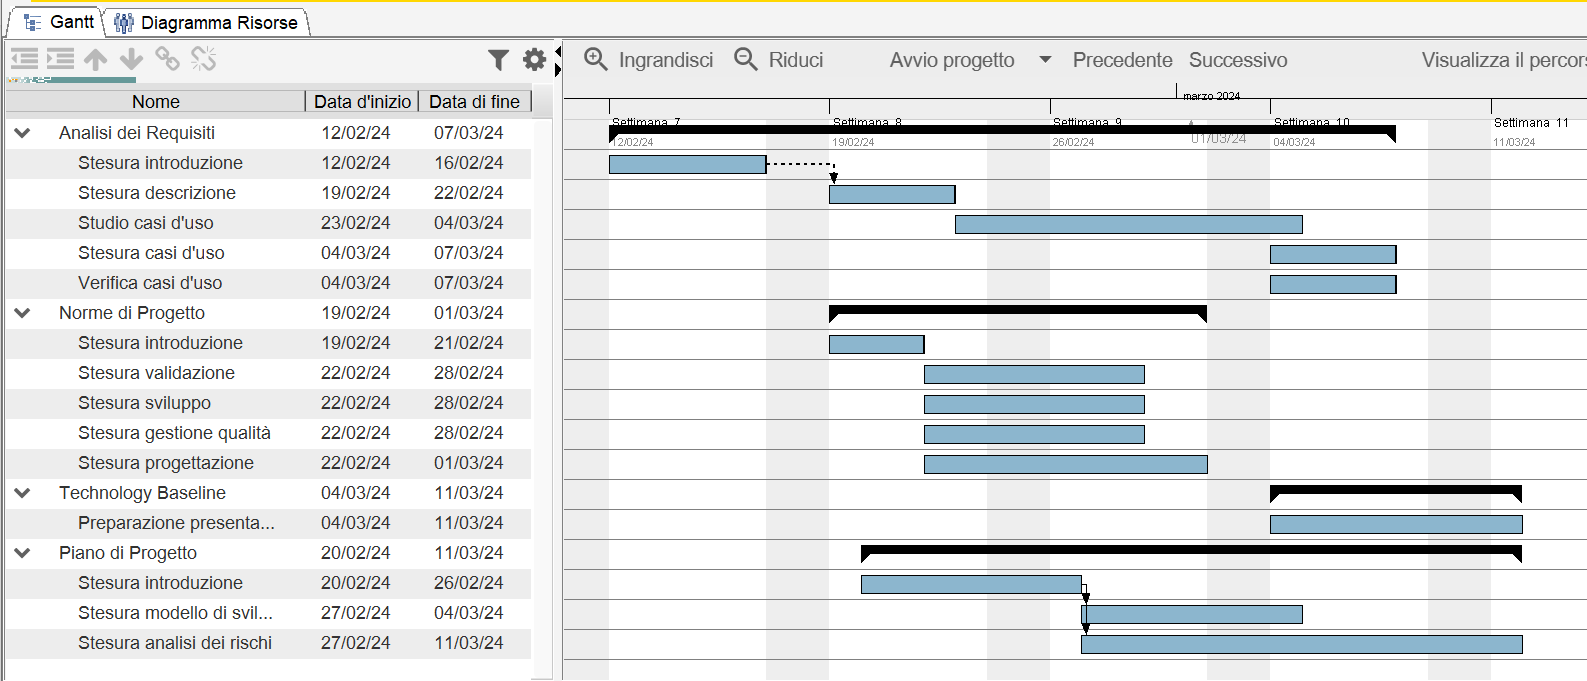
\includegraphics[scale=.6]{GanttTerzoPeriodo.png} \end{figure}

\pagebreak

\textbf{Consuntivo orario}

\begin{tblr}{
    colspec={|X[5cm]|X[.5cm]|X[.5cm]|X[.5cm]|X[.5cm]|X[.5cm]|X[.5cm]|X[3.5cm]},
    row{odd}={bg=white},
    row{even}={bg=lightgray},
    row{1}={bg=black,fg=white},
    row{8}={bg=black,fg=white}
    }
    
    Nominativo    & Re & Am & An & Pg & Pr & Vf & Ore Totali \\ \hline
    Alberto C.    & -  & 2  & 3  & -  & -  & -  & 5 \\ \hline
    Bibal El M.   & -  & -  & 2  & -  & -  & 3  & 5 \\ \hline
    Alberto M.    & -  & -  & 12 & -  & -  & 5  & 17 \\ \hline
    Alex S.       & -  & 5  & 10 & -  & -  & 5  & 20 \\ \hline
    Iulius S.     & -  & -  & 12 & -  & -  & 5  & 17  \\ \hline
    Giovanni Z.   & 5  & -  & 3  & -  & -  & 2  & 10 \\ \hline
    Totale        & 5  & 7  & 42 & 0  & 0  & 20 & 74 \\ \hline

\end{tblr}

\textbf{Consuntivo economico}

\begin{tblr}{
colspec={|X[5cm]|X[3.5cm]|X[1.5cm]|X[3.5cm]},
row{odd}={bg=white},
row{even}={bg=lightgray},
row{1}={bg=black,fg=white},
row{8}={bg=black,fg=white}
}

Ruolo & Costo orario (€/h) & N. Ore & Costo totale (€)  \\ \hline
Responsabile      & 30,00 &  5  &   150,00 \\ \hline
Amministratore    & 20,00 &  7  &   140,00 \\ \hline
Analista          & 25,00 &  42 &  1050,00 \\ \hline
Progettista       & 25,00 &   0 &     0,00 \\ \hline
Programmatore     & 15,00 &   0 &     0,00 \\ \hline
Verificatore      & 15,00 &  20 &   300,00 \\ \hline
Totale & \SetCell[c=1]{c} &  74 & 1.640,00 \\ \hline

\end{tblr}

\textbf{Gestione dei ruoli}

\paragraph{}
Nel terzo periodo, il 56\% delle risorse temporali del gruppo è stato speso nel ruolo dell'Analista,data la necessità 
di portare a compimento la stesura della prima versione dell'Analisi dei Requisiti in vista della prima fase della revisione
RTB; di conseguenza il gruppo ha utilizzato il 27\% delle ore per i processi di verifica e validazione del documento sopra citato, processi che
sono stati particolarmente attenzionati dai membri, vista l'importanza del documento stesso; inoltre il 9\% delle ore sono state dedicate alla figura dell'Amministratore
migrazione di tutta la documentazione sulla repository in GitHub e alla messa a punto della relativa gestione di configurazione,operazioni alle quali ha partecipato anche il Responsabile.

\pagebreak

\paragraph{Gestione dei rischi}

\begin{itemize}
\item \textbf{Rischio verificatosi:} Analisi incompleta/carente dei requisiti.
\begin{itemize}
\item \textbf{Esito Piano di Contingenza:} I membri del gruppo deputati alla stesura dell'Analisi dei Requisiti hanno constatato tardivamente
che i requisiti funzionali individuati prima del terzo periodo fossero insufficienti, in termini di numero e di 
profondità dell'analisi stessa; si è deciso quindi di destinare un maggior numero di ore a quest'ultima e di incrementare da
 2 a 3 il numero di componenti deputati ad essa. \\
\item \textbf{Impatto:} Significativo è stato l'impatto del suddetto rischio,avendo comportato la necessità
da parte del gruppo, di riallocare parte delle risorse orarie, dedicando 7 ore in più alla fase di analisi senza però
aumentare il monte orario complessivo preventivato all'inizio del terzo periodo; sono state
quindi tolte risorse alla stesura degli altri documenti.\\
\end{itemize}

\item \textbf{Rischio verificatosi:} Calcolo delle tempistiche.\\
\begin{itemize}
\item \textbf{Esito Piano di Contingenza:} In seguito al verificarsi del rischio legato ad una carente analisi dei requisiti, il Responsabile ha realizzato
che sarebbe stato necessario aumentare non solo le ore da dedicare all'analisi stessa, ma anche alla verifica e 
validazione delle sezioni del relativo documento, che venivano iterativamente prodotte e corrette; il gruppo è riuscito  a non aumentare
il monte orario preventivato all'inizio del terzo periodo. \\
\item \textbf{Impatto:} L'impatto è stato significativo; nonostante non direttamente misurabile in un aumento del monte orario preventivato,
si è tradotto in un'importante riallocazione di ore , tolte dal prosieguo della stesura della restante documentazione (in particolare del Piano
di Qualifica).
\end{itemize}

\item \textbf{Rischio verificatosi:} Disponibilità dei membri.
\begin{itemize}
    \item \textbf{Esito Piano di Contingenza:} In concomitanza dell'inizio della sessione d'esami, non è stato possibile una redistribuzione dei compiti dai membri
    con un numero maggiore di esami da sostenere a quelli meno impegnati; di comune accordo si è deciso quindi di interrompere fino al termine della sessione
    le attività del gruppo.
    \item \textbf{Impatto:} L'impatto è stato importante in quanto vi è stato un rallentamento eccessivo da parte di tutti i membri del gruppo,nonostante
    esso fosse stato preventivato; tale impatto è misurabile in un ritardo di 14 giorni rispetto alla tabella di marcia.
\end{itemize}
\end{itemize}

\paragraph{}
\textbf{Retrospettiva:} \\
Nel terzo periodo, essendo stata completata la codifica del PoC, il gruppo ha speso la maggior parte dell proprie risorse per proseguire la stesura dei documenti, con attenzione
particolare nei confronti dell'Analisi dei Requisiti data la volontà di recuperare parte del ritardo accumulato sulla tabella di marcia e di voler effettuare la prima parte dell'RTB;
purtroppo, come avvenuto nel secondo periodo, il ritmo di lavoro ha subito un nuovo rallentamento a causa della sessione invernale di esami, rendendo evidente da parte del gruppo una 
parziale incapacità di mettere in atto un efficiente piano di contingenza con i rischi di una scarsa comunicazione e di una fallace pianificazione; data l'importanza dell'Analisi
dei Requisiti, si è reso necessario concentrare in essa buona parte delle risorse orarie, rallentando così la stesura degli altri documenti.
\begin{itemize} 
    \item \textbf{Obiettvi raggiunti:}
    \begin{itemize}
        \item Stesura della prima versione dell'Analisi dei Requisiti;
        \item Inizio della stesura del Piano di Qualifica;
        \item Inizio della stesura del Glossario;
        \item Prosieguo della stesura delle Norme e del Piano di Progetto;
        \item Creazione di uno script per la verifica automatica dei documenti.
    \end{itemize}
    \item \textbf{Obiettivi mancati:}
    \begin{itemize}
        \item Stesura della prima versione delle Norme di Progetto;
        \item Stesura della prima versione del Piano di Progetto.
    \end{itemize}
\end{itemize}

\subsubsection{Quarto periodo} 
Inizio: 12/03/2024 \\
Fine: ?? \\

\textbf{Preventivo orario}

\begin{tblr}{
    colspec={|X[5cm]|X[.5cm]|X[.5cm]|X[.5cm]|X[.5cm]|X[.5cm]|X[.5cm]|X[3.5cm]},
    row{odd}={bg=white},
    row{even}={bg=lightgray},
    row{1}={bg=black,fg=white},
    row{8}={bg=black,fg=white}
    }
    
    Nominativo    & Re & Am & An & Pg & Pr & Vf & Ore Totali \\ \hline
    Alberto C.    & -  & -  & -  & 2  & -  & 3  & 5 \\ \hline
    Bibal El M.   & 2  & 2  & 4  & 2  & -  & 5  & 15 \\ \hline
    Alberto M.    & -  & -  & 4  & -  & -  & 5  & 9 \\ \hline
    Alex S.       & 2  & 3  & -  & -  & -  & -  & 5 \\ \hline
    Iulius S.     & -  & -  & 4  & -  & -  & 5  & 9  \\ \hline
    Giovanni Z.   & -  & -  & -  & 5  & -  & 5  & 10 \\ \hline
    Totale        & 4  & 5  & 12 & 9  & 0  & 23 & 53 \\ \hline

\end{tblr}

\textbf{Preventivo economico}

\begin{tblr}{
colspec={|X[5cm]|X[3.5cm]|X[1.5cm]|X[3.5cm]},
row{odd}={bg=white},
row{even}={bg=lightgray},
row{1}={bg=black,fg=white},
row{8}={bg=black,fg=white}
}

Ruolo & Costo orario (€/h) & N. Ore & Costo totale (€)  \\ \hline
Responsabile      & 30,00 &  4  &   120,00 \\ \hline
Amministratore    & 20,00 &  5  &   100,00 \\ \hline
Analista          & 25,00 &  12 &   300,00 \\ \hline
Progettista       & 25,00 &  9  &   225,00 \\ \hline
Programmatore     & 15,00 &   0 &     0,00 \\ \hline
Verificatore      & 15,00 &  23 &   345,00 \\ \hline
Totale & \SetCell[c=1]{c} &  53 & 1.090,00 \\ \hline

\end{tblr}

\textbf{Attività svolte}

\paragraph{}
Le attività svolte dal gruppo nel quarto periodo sono state:
\begin{itemize}
    \item Modifica dell'Analisi dei Requisiti e correzione degli errori come indicato dal prof. Cardin;
    \item Completamento della sezione "Pianificazione" del Piano di Progetto;
    \item Completamento della stesura del Piano di Qualifica;
    \item Completamento delle Norme di Progetto;
    \item Creazione di uno script per automatizzare l'operazione di individuazione dei termini presenti nei vari documenti,
    da inserire nel Glossario;
    \item Stesura della prima versione del Glossario;
    \item Consuntivo finale della fase RTB;
    \item Preparazione della presentazione per la seconda fase della RTB.
\end{itemize}

%Da aggiungere diagrammi di Gantt realtivi al quarto periodo

\textbf{Consuntivo orario}

\begin{tblr}{
    colspec={|X[5cm]|X[.5cm]|X[.5cm]|X[.5cm]|X[.5cm]|X[.5cm]|X[.5cm]|X[3.5cm]},
    row{odd}={bg=white},
    row{even}={bg=lightgray},
    row{1}={bg=black,fg=white},
    row{8}={bg=black,fg=white}
    }
    
    Nominativo    & Re & Am & An & Pg & Pr & Vf & Ore Totali \\ \hline
    Alberto C.    & -  & -  & -  & 2  & -  & 3  & 5 \\ \hline
    Bibal El M.   & 2  & -  & 4  & 2  & -  & 5  & 13 \\ \hline
    Alberto M.    & -  & -  & 4  & -  & -  & 5  & 9 \\ \hline
    Alex S.       & 5  & 5  & -  & -  & -  & -  & 10 \\ \hline
    Iulius S.     & -  & -  & 4  & -  & -  & 5  & 9  \\ \hline
    Giovanni Z.   & -  & -  & -  & 5  & -  & 5  & 10 \\ \hline
    Totale        & 7  & 5  & 12 & 9  & -  & 23 & 56 \\ \hline

\end{tblr}

\textbf{Consuntivo economico}

\begin{tblr}{
colspec={|X[5cm]|X[3.5cm]|X[1.5cm]|X[3.5cm]},
row{odd}={bg=white},
row{even}={bg=lightgray},
row{1}={bg=black,fg=white},
row{8}={bg=black,fg=white}
}

Ruolo & Costo orario (€/h) & N. Ore & Costo totale (€)  \\ \hline
Responsabile      & 30,00 &  7  &   210,00 \\ \hline
Amministratore    & 20,00 &  5  &   100,00 \\ \hline
Analista          & 25,00 &  12 &   300,00 \\ \hline
Progettista       & 25,00 &   9 &   225,00 \\ \hline
Programmatore     & 15,00 &   0 &     0,00 \\ \hline
Verificatore      & 15,00 &  23 &   345,00 \\ \hline
Totale & \SetCell[c=1]{c} &  56 & 1.180,00 \\ \hline

\end{tblr}

\textbf{Gestione dei ruoli}

\paragraph{}
Come si può vedere dalla suddetta tabella,in questo quarto periodo il gruppo ha concentrato buona parte del monte-ore nello svolgimento
del ruolo di Analista e soprattutto di Verificatore: per quanto concerne il primo, i membri hanno speso il 21\% delle risorse al fine di completare la stesura di tutta la documentazione e di effettuare le correzioni all'Analisi dei Requisiti
in seguito alla revisione del prof. Cardin; in previsione della seconda fase della RTB, una parte cospicua di risorse (\%50) è stata utilizzata per la fase di verifica 
e validazione della documentazione sopracitata; il gruppo ha inoltre riservato il 12\% delle ore al ruolo del Responsabile, data l'importanza di un efficace
ed efficiente orchestrazione delle attività del gruppo in vista della seconda parte della RTB, e il 9\% di ore alla figura dell'Amministratore, al fine
di evitare potenziali conflitti negli items di versionamento prodotti dai differenti membri; infine, il 16\% delle risorse è stato dedicato al Progettista.

\paragraph{Gestione dei rischi}

\begin{itemize}
    \item \textbf{Rischio verificatosi:} Conflitti decisionali.
    \begin{itemize}
        \item \textbf{Esito Piano di Contingenza:}In seguito alla revisione della Technology Baseline effettuate dal prof. Cardin, sono emerse criticità nella progettazione
        del PoC e in particolare nella scelta dello stack tecnologico; è stata quindi avviata una discussione tra i membri del gruppo su come risolvere tali criticità,
        consci della tabella di marcia da seguire rigorosamente al fine di completare la revisione PB evitando ulteriore ritardo a quello già accumulato. Data la 
        natura sensibile dell'oggetto della discussione, i membri hanno faticato più del previsto a trovare una soluzione condivisa da tutti.
        \item \textbf{Impatto:} L'impatto dei conflitti decisionali riguardanti eventuali modifiche dello stack tecnologico non è ancora misurabile, poichè non è
        prevedibile allo stato attuale  se avverrà una modifica dello stack, e in caso quest'ultima avvenga, una misura quantitativa delle risorse che il gruppo dovrà
        forzatamente riallocare.
    \end{itemize}
\end{itemize}

\textbf{Retrospettiva:} \\
Come si evince dalla tabella del consuntivo orario, in questo quarto periodo il gruppo si è prodigato nel terminare la stesura di tutta la documentazione restante,
e nelle successive operazioni di verifica e validazione; in seguito alla revisione TB effettuata dal prof. Cardin, sono state apportate le necessario modifiche all'Analisi
dei Requisiti.Inoltre, a seguito delle perplessità espresse dal prof. Cardin riguardo le scelte riguardo lo stack tecnologico, il gruppo si è visto costretto a dedicare parte delle risorse ad 
un nuovo lavoro di studio e ricerca per capire se includere nuovi framework o linguaggi nello stack tecnologico, soprattutto in previsione della progettazione dell'MVP.
\begin{itemize} 
    \item \textbf{Obiettvi raggiunti:}
    \begin{itemize}
        \item Stesura della prima versione delle Norme di Progetto;
        \item Stesura della prima versione del Piano di Progetto;
        \item Stesura della prima versione del Piano di Qualifica;
        \item Creazione di uno script per l'individuazione di tutti i termini facenti parte del Glossario;
        \item Stesura della prima versione del Glossario;
        \item Candidatura per la seconda parte dell'RTB;
        \item Stesura della seconda versione dell'Analisi dei Requisiti.
    \end{itemize}
    \item \textbf{Obiettivi mancati:}
    \begin{itemize}
        \item Nessuno.
    \end{itemize}
\end{itemize}

\subsubsection{Riepilogo finale}
\textbf{Preventivo economico totale}

\begin{tblr}{
    colspec={|X[5cm]|X[3.5cm]|X[1.5cm]|X[3.5cm]},
    row{odd}={bg=white},
    row{even}={bg=lightgray},
    row{1}={bg=black,fg=white},
    row{8}={bg=black,fg=white}
    }
    
    Ruolo & Costo orario (€/h) & N. Ore & Costo totale (€)  \\ \hline
    Responsabile      & 30,00 &  21 &   630,00 \\ \hline
    Amministratore    & 20,00 &  18 &   360,00 \\ \hline
    Analista          & 25,00 &  67 &  1675,00 \\ \hline
    Progettista       & 25,00 &  26 &   650,00 \\ \hline
    Programmatore     & 15,00 &  30 &   450,00 \\ \hline
    Verificatore      & 15,00 &  49 &   735,00 \\ \hline
    Totale & \SetCell[c=1]{c} & 211 &  4500,00 \\ \hline
    
    \end{tblr}

\textbf{Consuntivo economico finale}

\begin{tblr}{
    colspec={|X[5cm]|X[3.5cm]|X[1.5cm]|X[3.5cm]},
    row{odd}={bg=white},
    row{even}={bg=lightgray},
    row{1}={bg=black,fg=white},
    row{8}={bg=black,fg=white}
    }
    
    Ruolo & Costo orario (€/h) & N. Ore & Costo totale (€)  \\ \hline
    Responsabile      & 30,00 &  19 &   570,00 \\ \hline
    Amministratore    & 20,00 &  20 &   400,00 \\ \hline
    Analista          & 25,00 &  70 &  1750,00 \\ \hline
    Progettista       & 25,00 &  30 &   750,00 \\ \hline
    Programmatore     & 15,00 &  40 &   600,00 \\ \hline
    Verificatore      & 15,00 &  61 &   915,00 \\ \hline
    Totale & \SetCell[c=1]{c} & 240 &  4985,00 \\ \hline
    
    \end{tblr}

\textbf{Preventivo orario totale}

\begin{tblr}{
    colspec={|X[5cm]|X[.5cm]|X[.5cm]|X[.5cm]|X[.5cm]|X[.5cm]|X[.5cm]|X[3.5cm]},
    row{odd}={bg=white},
    row{even}={bg=lightgray},
    row{1}={bg=black,fg=white},
    row{8}={bg=black,fg=white}
    }
    
    Nominativo    & Re & Am & An & Pg & Pr & Vf & Ore Totali \\ \hline
    Alberto C.    & -  & -  & 5  & 6  & 15 & 6  & 32 \\ \hline
    Bibal El M.   & 4  & 5  & 13 & 6  & -  & 15 & 43 \\ \hline
    Alberto M.    & 8  & 2  & 19 & -  & -  & 7  & 36 \\ \hline
    Alex S.       & 4  & 11 & 5  & 5  & 5  & 5  & 35 \\ \hline
    Iulius S.     & -  & -  & 25 & -  & -  & 10 & 35 \\ \hline
    Giovanni Z.   & 5  & -  & -  & 9  & 10 & 6  & 30 \\ \hline
    Totale        & 21 & 18 & 67 & 26 & 30 & 49 & 211\\ \hline

\end{tblr}

\textbf{Consuntivo orario finale}

\begin{tblr}{
    colspec={|X[5cm]|X[.5cm]|X[.5cm]|X[.5cm]|X[.5cm]|X[.5cm]|X[.5cm]|X[3.5cm]},
    row{odd}={bg=white},
    row{even}={bg=lightgray},
    row{1}={bg=black,fg=white},
    row{8}={bg=black,fg=white}
    }
    
    Nominativo    & Re & Am & An & Pg & Pr & Vf & Ore Totali \\ \hline
    Alberto C.    & -  & 2  & 3  & 6  & 20 & 9  & 40\\ \hline
    Bibal El M.   & 2  & -  & 10 & 6  & -  & 11 & 29\\ \hline
    Alberto M.    & 5  & 5  & 21 & -  & -  & 10 & 41\\ \hline
    Alex S.       & 7  & 13 & 10 & 5  & 5  & 10 & 50\\ \hline
    Iulius S.     & -  & -  & 23 & 4  & -  & 13 & 40\\ \hline
    Giovanni Z.   & 5  & -  & 3  & 9  & 15 & 8  & 40\\ \hline
    Totale        & 19 & 20 & 70 & 30 & 40 & 61 & 240\\ \hline

\end{tblr}

\textbf{Gestione dei ruoli} \\
Durante la fase di RTB, il 29\% delle risorse orario è stato dedicato al ruolo di Analista, il 17\% a quello di Programmatore, il 25\% a quello di Verificatore,mentre
solo l'8 \%  per le figure rispettivamente del Responsabile e dell'Amministratore; il 13\% per la figura del Progettista.
\textbf{Restrospettiva finale}
Analizzando le gestione da parte del gruppo dei ruoli, salta subito all'occhio un forte sbilanciamento, in parte abbastanza naturale nella fase di RTB, a favore di alcuni ruoli a discapito di altri: abbondanti risorse sono state spese
per la figura dell'Analista in quanto la produzione dei documenti in generale , e dell'Analisi dei Requisiti in particolare, si è dimostrata un compito assai più oneroso di quanto si fosse preventivato
inizialmente; di questo fatto, è considerata una diretta conseguenza la quantità di risorse dedicate alla verifica e alla validazione della documentazione e del codice del PoC. Il gruppo riconosce retrospettivamente 
che troppe poche risorse sono state dedicate in primis alla figura del Responsabile: un'attenzione evidentemente non sufficiente ai compiti di gestione del gruppo (soprattutto per quanto riguarda la comunicazione),di assegnazione
dei compiti (che ha comportato una differenza importante nella quantità di lavoro proffuso da alcuni membri) e
di coordinamento delle risorse impiegate, è considerata dai membri una delle cause principali delle molteplici criticità emerse durante tutta la RTB. 
%cosa mettere?  Gestione ruoli di tutta la RTB? Retrospettiva totale, anche sui difetti? Spiegare le differenze di ore? Perchè tanta analisi?
% Previsione per la PB : molte + ore per il progettista,per i programmatori e per i verificatori;
\subsection{Verso la PB}

Sono di seguito presenti le tabelle, rispettivamente, delle ore preventivate di lavoro che ogni membro dedicherà al progetto durante la fase PB, e del Costo
totale che il gruppo spenderà per la suddetta fase. Per quanto concerne il preventivo orario, le ore sono state allocate tra i membri del gruppi facendo in modo
che ognuno ne abbia speso 85 dall'inizio del progetto e abbia svolto almeno una volta ogni ruolo (durante la fase RTB, non tutti i membri del gruppo ne hanno avuto la
possibilità).

\textbf{Preventivo orario PB}

\begin{tblr}{
    colspec={|X[5cm]|X[.5cm]|X[.5cm]|X[.5cm]|X[.5cm]|X[.5cm]|X[.5cm]|X[3.5cm]},
    row{odd}={bg=white},
    row{even}={bg=lightgray},
    row{1}={bg=black,fg=white},
    row{8}={bg=black,fg=white}
    }
    
    Nominativo    & Re & Am & An & Pg & Pr & Vf & Ore Totali \\ \hline
    Alberto C.    & 5  & -  & 5  & 5  & 20 & 10 & 45\\ \hline
    Bibal El M.   & -  & 5  &  - & 5  & 25 & 21 & 56\\ \hline
    Alberto M.    & 5  & -  &  - & 10 & 20 &  9 & 44\\ \hline
    Alex S.       & 10 & 5  &  - & 10 & -  & 10 & 35\\ \hline
    Iulius S.     & 5  & 5  &  - & 5  & 20 & 10 & 45\\ \hline
    Giovanni Z.   & 5  & 5  & 5  & 5  & 15 & 10 & 40\\ \hline
    Totale        & 30 & 20 & 10 & 40 & 100& 70 & 270\\ \hline

\end{tblr}

\textbf{Preventivo economico PB}

\begin{tblr}{
    colspec={|X[5cm]|X[3.5cm]|X[1.5cm]|X[3.5cm]},
    row{odd}={bg=white},
    row{even}={bg=lightgray},
    row{1}={bg=black,fg=white},
    row{8}={bg=black,fg=white}
    }
    
    Ruolo & Costo orario (€/h) & N. Ore & Costo totale (€)  \\ \hline
    Responsabile      & 30,00 &  30 &   900,00 \\ \hline
    Amministratore    & 20,00 &  20 &   400,00 \\ \hline
    Analista          & 25,00 &  10 &   250,00 \\ \hline
    Progettista       & 25,00 &  40 &  1000,00 \\ \hline
    Programmatore     & 15,00 & 100 &  1500,00 \\ \hline
    Verificatore      & 15,00 &  70 &  1050,00 \\ \hline
    Totale & \SetCell[c=1]{c} & 270 &  5100,00 \\ \hline
    
    \end{tblr}

Come si può vedere dalla tabella del preventivo economico, il totale con il consuntivo della fase RTB è di 10.085 euro, in linea quindi
con il preventivo presentato dal gruppo ad inizio progetto di 10.980 euro; per quanto riguarda la conclusione del progetto, il gruppo è costretto,
a fronte del significativo ritardo accumulato durante la fase RTB, a posticiparne la data al 15 Giugno.